%-----------------------------------------------------------------------------
%
%               Template for sigplanconf LaTeX Class
%
% Name:         sigplanconf-template.tex
%
% Purpose:      A template for sigplanconf.cls, which is a LaTeX 2e class
%               file for SIGPLAN conference proceedings.
%
% Guide:        Refer to "Author's Guide to the ACM SIGPLAN Class,"
%               sigplanconf-guide.pdf
%
% Author:       Paul C. Anagnostopoulos
%               Windfall Software
%               978 371-2316
%               paul@windfall.com
%
% Created:      15 February 2005
%
%-----------------------------------------------------------------------------


\documentclass[preprint]{sigplanconf}

% The following \documentclass options may be useful:
%
% 10pt          To set in 10-point type instead of 9-point.
% 11pt          To set in 11-point type instead of 9-point.
% authoryear    To obtain author/year citation style instead of numeric.

\usepackage{amsmath}
\usepackage{graphicx}

\begin{document}

\conferenceinfo{WXYZ '05}{date, City.} 
\copyrightyear{2005} 
\copyrightdata{[to be supplied]} 

\titlebanner{banner above paper title}        % These are ignored unless
\preprintfooter{short description of paper}   % 'preprint' option specified.

\title{iMonitor: An Implicit-Signal Monitor}
\subtitle{}

\authorinfo{Wei-Lun Hung}
{Dept. of Electrical and Computer Engineering, \\ 
  The University of Texas at Austin.}
{wlhung@utexas.edu}
\authorinfo{Vijay K. Garg}
{Dept. of Electrical and Computer Engineering, \\ 
  The University of Texas at Austin.}
{garg@ece.utexas.edu}

\maketitle

\begin{abstract}
  This is the text of the abstract.
\end{abstract}

\category{CR-number}{subcategory}{third-level}

\terms
term1, term2

\keywords
keyword1, keyword2

\section{Introduction}

The text of the paper begins here.

\section{Background}
\section{Syntax and Framework of iMonitor}


\begin{table}
  \begin{tabular}{| l | l | }
    \hline
    class BoundedBuffer \{ & 
      monitor class BoundedBuffer \{ \\
    \ \ int[] items;  & 
      \ \   int[] items; \\
    \ \ condition not\_full, not\_empty; & 
      \ \ int putptr, takeptr, count; \\
    \ \ int putptr, takeptr, count; & 
      \ \ public BoundedBuffer(int n) \{ \\
    \ \ public BoundedBuffer(int n) \{ &  
      \ \ \ \ putptr = takeptr = count = 0; \\
    \ \ \ \ putptr = takeptr = count = 0; & 
      \ \ \ \ items = new int[n]; \\
    \ \ \ \ items = new int[n]; & 
      \ \ \} \\
    \ \ \} & 
      \ \ public void put(int x) \{ \\
    \ \ public void put(int x) \{ & 
      \ \ \ \ waituntil(count < items.length); \\
    \ \ \ \ if(count == items.length) \{ &
      \ \ \ \ int x = items[putptr] = x; \\
    \ \ \ \ \ \ not\_full.await(); & 
      \ \ \ \ if(++putptr == items.length) \{ \\
    \ \ \ \ \} &  
      \ \ \ \ \ \ putptr = 0; \\
    \ \ \ \ int x = items[putptr] = x; & 
      \ \ \ \ \} \\
    \ \ \ \ if(++putptr == items.length) \{ & 
      \ \ \ \ ++count; \\
    \ \ \ \ \ \ putptr = 0; & 
      \ \ \} \\
    \ \ \ \ \} &
      \ \ public int take() \{ \\
    \ \ \ \ ++count; &
      \ \ \ \ waituntil(count $>$ 0); \\
    \ \ \ \ not\_empty.signal(); &
      \ \ \ \ int x = items[takeptr]; \\
    \ \ \} &
      \ \ \ \ if(++takeptr == items.length) \{ \\
    \ \ public int take() \{ &
      \ \ \ \ \ \ takeptr = 0; \\
    \ \ \ \ if(count == 0) \{ &
      \ \ \ \ \} \\
    \ \ \ \ \ \ not\_empty.await(); & 
      \ \ \ \ return x; \\
    \ \ \ \ \} &
      \ \ \} \\
    \ \ \ \ int x = items[takeptr]; &
      \} \\
    \ \ \ \ if(++takeptr == items.length) \{ & \\ 
    \ \ \ \ \ \ takeptr = 0; & \\
    \ \ \ \ \} & \\
    \ \ \ \ not\_full.signal(); & \\
    \ \ \ \ return x; & \\
    \ \ \} & \\
    \} & \\
    \hline
  \end{tabular}
\end{table}
\begin{figure}[h!]
  \centering
  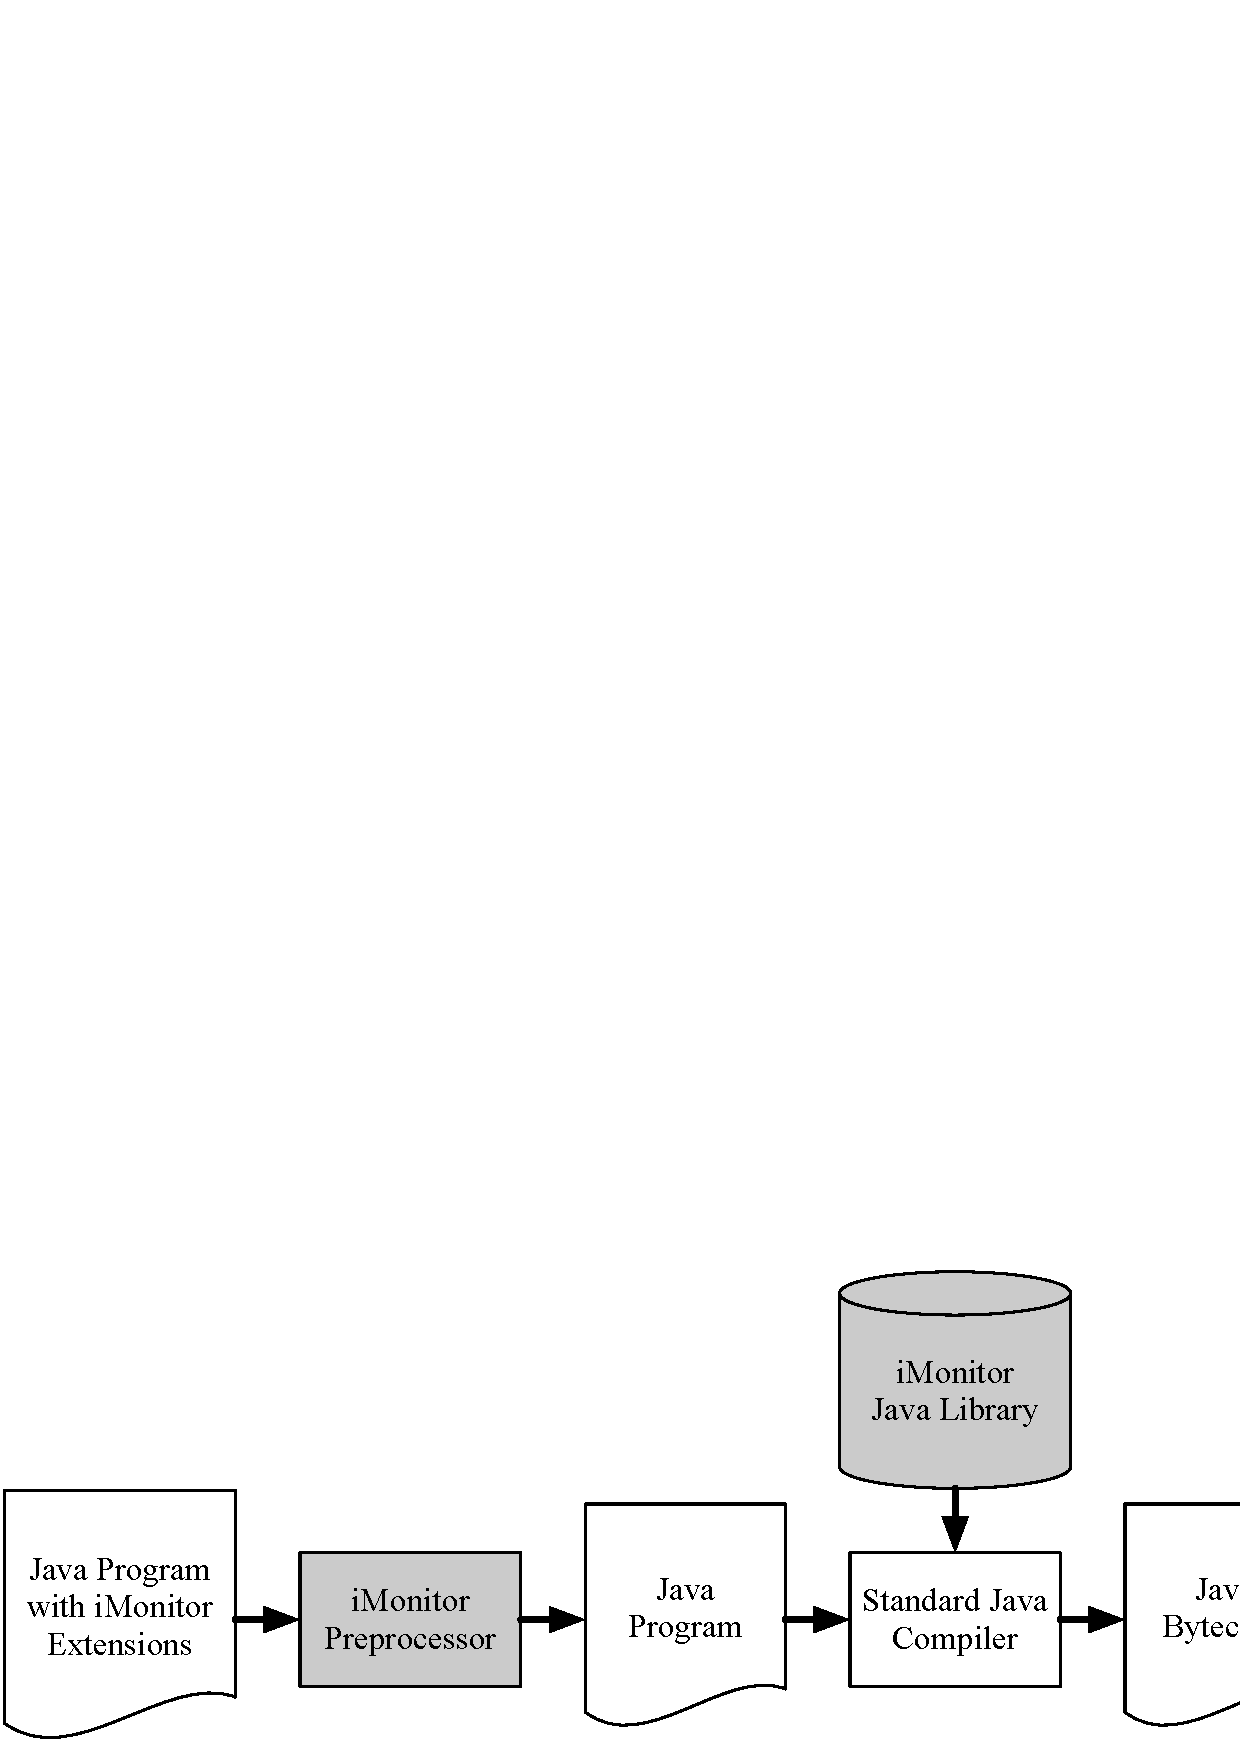
\includegraphics[width=70mm]{fig/flow.png}
  \caption{The framework of iMonitor}
  \label{fig:framework}
\end{figure}

monitor variables (class variables)


\section{Details of Implicit-Signal Monitors}
The implementation of the implicit-signal monitor in iMonitor involves four 
parts:

\begin{enumerate}
  \item Monitor-constructor: the constructor of the monitor class, including 
    definitions and declarations of additional variables to provide mutual 
    exclusion and synchronization of monitor. 
  \item Monitor-function entry: executed before each member function, 
    involving declarations of additional variables and code to maintain
    mutual exclusion of monitor. 
  \item Monitor-waituntil statement: including declarations of additional
    variables and signal/await statements to implement the waituntil.
  \item Monitor-function leave: executed before the return statement of 
    each member function, involving code to guarantee mutal exclusion and 
    synchronization of monitor. 
\end{enumerate}



\subsection{Naive}

\begin{table}
  \center
  \begin{tabular}{| l || l |}
    \hline
    constructor & Lock mutex; \\
                & Condition cond; \\
    \hline
    entry & mutex.lock(); \\
    \hline
    waituntil C & if(!C) \{  \\
                & \ \ cond.signalAll(); \\
                & \ \ do \{ \\
                & \ \ \ \ cond.await(); \\
                & \ \ \}  while(!C); \\
                & \} \\
    \hline
    exit & mutex.unlock(); \\
         & cond.signalAll(); \\
    \hline
  \end{tabular}
  \caption{Naive monitor implementation}
  \label{tab:naive_imp}
\end{table}

The implementation of naive implicit-signal monitor is shown in Table 
\ref{tab:naive_imp}. One lock variable, {\bf \it mutex}, is declared for 
mutual exclusion, which should be acquired in the begining of every member 
function and released before the return statement. In addition, one condition
variable, {\bf \it cond}, is declared for synchronization, 

\subsection{N-Condition}

\subsection{HashMap-Condition}
\subsection{Dependent-Condition} 
\section{Experimental Results}
\subsection{Bounded-Buffer Problem}
\subsection{Reader/Writer Problem}
\subsection{Dining Philosophers  Problem}
\subsection{Sleeping Barber Problem}
\subsection{Access Patterns}

\section{Conclusions}

\appendix
\section{Appendix Title}

This is the text of the appendix, if you need one.

\acks

Acknowledgments, if needed.

% We recommend abbrvnat bibliography style.

\bibliographystyle{abbrvnat}

% The bibliography should be embedded for final submission.

\begin{thebibliography}{}
    \softraggedright

  \bibitem[Buhr et~al.(2005)Buhr, P.A.]{bh05}
    Buhr, P. A. and Harji, A. S. Implicit-Signal Monitors. ACM Transactions on Programming Languages and Systems, 27(6), 1270�1343. ACM. doi:10.1145/1108970.1108975

\end{thebibliography}

\end{document}
